\chapter{Videospielentwicklung}

Jedes Videospiel hat seine eigenen Regeln, die ein Videospielentwickler �ber eine bestimmte Programmiersprache entwickelt. So wurde beispielsweise das Arcade-Videospiel �Marble Madness� (1984) von Atari Games in C programmiert. Zuvor programmierte Atari Games ihre Spiele in Assemblersprache. Die heutigen Spielwelten werden von Game-Developern mithilfe einer Game-Engine entwickelt.

\section{Game-Engines}

Mit der Zeit wuchs die Komplexit�t und Kosten von Videospielen, was zu Game-Engines f�hrte. Eine Game-Engine ist eine Entwicklungsumgebung in welcher Videospiele programmiert und zusammengestellt werden. Zu Beginn wurden Game-Engines f�r bestimmte Videospiele geschrieben, die jedoch f�r �hnliche Videospiele weiterverwendet wurden. So hat beispielsweise id Software ihre Videospiel-Serie �Commander Keen� (1990) als Game-Engine programmiert, was die Entwicklungszeit der Commander Keen -Reihe verk�rzte und die Game-Engine im Jahr 1991 lizensiert.  Eine weitere bekanntere Game-Engine ist die Doom-Engine (id Tech), welche ebenfalls von id Software stammt und f�r das Videospiel Doom (1993) programmiert wurde. Die Doom-Engine hat dabei ein minimalistisches Ma� an Programmierbarkeit geboten. Benutzer konnten in der Game-Engine Daten in einem vorgegebenen Format hinzuf�gen. Die daraus entstandenen Spielwelten hatten dabei andere Layouts spielten sich aber wie Doom.\\
In heutiger Zeit sind Game-Engines ein Sofware-Programm mit einer Kollektion an Modulen, welche der Spieleentwickler zur Entwicklung seines Videospiels nutzt. Die Gr��e der Game-Engine variiert nach der Anzahl an Funktionen, welche durch bestimmte Module umgesetzt werden. Typische Funktionen w�ren: das Rendern von Grafiken, Verarbeitung von Eingaben �ber Eingabeger�te, Umsetzung von Physik und Kollisionen, Audio-Ausgabe oder Netzwerk-Funktionen f�r die Umsetzung online mit anderen Spielern zu spielen. Eine Game-Engine kann auch software development kits (SDKs) integrieren, so kann beispielsweise die Funktion der Umsetzung immersiver Physik und Kollision durch die Havok SDK umgesetzt werden.\\
Die Wahl einer bestimmten Game-Engine h�ngt von dem jeweiligen Genre oder spezifischen Anforderungen des zu entwickelnden Videospiels ab. Zu den aktuelle Game-Engines z�hlen: Unity, Unreal, Cry-Engine, RPGMaker, GameMaker oder Godot. W�hrend sich beispielsweise die RPGMaker-Engine auf das Genre der Rollenspiele spezialisiert, liegt der Fokus der Unreal-Engine auf der Entwicklung grafisch realistischer 3D-Videospiele.

\section{Game-AI}

Spieleentwickler nutzen akademische Forschungen aus dem Bereich der AI, um Algorithmen zu entwickeln, welche Agenten der Spielwelt \textit{Non-Player Character (NPC)} ein menschlicheres oder tierischeres Verhalten verleihen. Eine Spielwelt beinhaltet statische und dynamische Entit�ten, wie NPC welche die Spielwelt immersiv machen. Die NPC, werden im Gegensatz zur Spielfigur vom Computer gesteuert. Ein NPC kann der Spielfigur je nach Narrativ freundlich, neutral oder feindlich interagieren. Ein Beispiel f�r feindliche NPC sind die Geister aus Pac-Man. Darin versuchten die Geister die Spielfigur in der Spielwelt zu fangen.\\
Die AI im Videospiel Bereich l�sst dabei in drei Bereiche unterteilen: Bewegung (\textit{Movement}), Entscheidungsfindung (\textit{Decision making}) und Strategie (\textit{Strategy}). Bewegung und Entscheidungsfindung beziehen sich dabei auf einzelne NPC, w�hrend Strategie-AI auf Gruppen von NPC (\textit{Group AI}) angewendet wird. Nicht alle Videospiele ben�tigen alle der drei genannten Bereiche. So ben�tigt Schach keine AI f�r Bewegung oder Entscheidungsfindung, sondern ausschlie�lich f�r Strategie.

\begin{figure}[h]
  \centering
  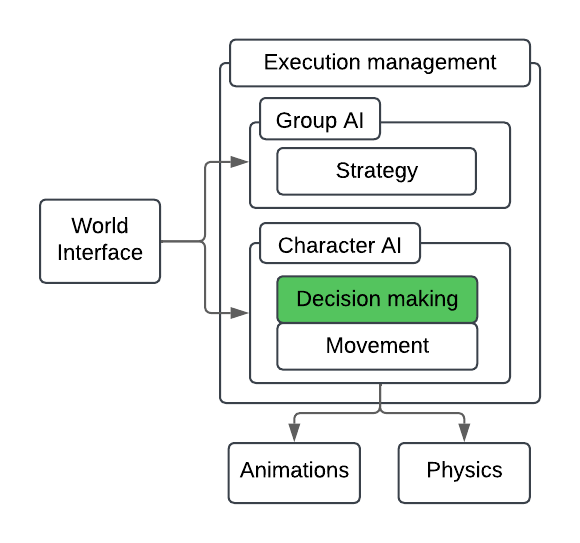
\includegraphics[width=9cm]{Videospielentwicklung/Game AI Diagramm}
	\captionsetup{justification=justified, format=plain}
  \caption{Game-AI Model: Die Thesis fokussiert sich auf den Bereich der Entscheidungsfindung (\textit{Decisionmaking}) in gr�n markiert}
  \label{Game AI}
\end{figure}

Der Bereich der Bewegungs-AI arbeitet haupts�chlich mit Algorithmen, die daf�r sorgen, dass ein NPC von einer Position in zur n�chsten gelangt, Hindernissen ausweicht oder den optimalen Pfad zu einem Ziel findet.\\
Eine Strategie-AI sorgt f�r die Koordination einer ganzen Gruppe von NPC. Die Strategie-AI soll dabei die Entscheidungsfindung der NPC beeinflussen. Beispielsweise hat die Strategie-AI des FPS Half-Life die feindlichen NPC dazu gebracht Spielerfigur zu flankieren.